\section{Cross-Domain Instantiation: Slime Mold and Transformer}

\subsection{Overview}

\S{}3 introduced the three minimal axioms, and \S{}4 introduced IFGT as a vocabulary for describing them. This section tests the substrate-independence of that structure by comparing two radically different systems: the biological network dynamics of \emph{Physarum polycephalum} and the layer dynamics of Transformer architectures.

The claim is structural homology only. The paper does not claim that slime mold thinks, that Transformers understand, or that the two systems are cognitively identical. The claim is that both instantiate the same minimal structural conditions in different substrates.

\subsection{The slime mold as an externally validated instantiation}

The tube-network dynamics of slime mold has been studied independently of the present framework. Nakagaki et al. (2000) reported maze-solving behavior without attributing intelligence as a possessed property \citep{Nakagaki2000}. Kobayashi, Tero, and Nakagaki (2006) modeled rhythmic protoplasmic motion \citep{Kobayashi2006}. Tero, Kobayashi, and Nakagaki (2007) formulated the Physarum solver as flow reinforcement plus decay \citep{Tero2007}.

The slime mold case can be mapped onto the three axioms:

\textbf{Connected state space.}
The tube network \(\{N_i,e_{ij}\}\) forms a connected graph. Nodes are nutrient sources or branching points. Edges are pathways for material and signal flow. Kirchhoff-style flow conservation gives the network dynamic connectedness.

\textbf{Temporal ordering.}
Conductivity evolves through
\[
\frac{dD_{ij}}{dt}=f(|Q_{ij}|)-D_{ij}.
\]
Past flow leaves a trace in present conductivity. This gives the system history.

\textbf{Global constraint.}
The global bias \(\Phi_{\mathrm{bio}}\) is supplied by nutrient sources, boundary conditions, energetic costs, and Kirchhoff constraints. Local flow reinforcement alone does not produce the final global structure. A global constraint is required.

\subsection{The Transformer as an artificial instantiation}

Transformers are not introduced here because of their engineering success or cognitive interpretation, but because their structure gives a clear artificial contrast case \citep{Vaswani2017}.

\textbf{Connected state space.}
For a token sequence, the state space is represented by hidden vectors
\[
\mathcal{S}=\{h_i^{(\ell)}\}.
\]
Attention connects token positions relationally. The connectedness is computational rather than biological, but it satisfies the structural condition of reachability through relations.

\textbf{Temporal ordering.}
Layer updates are ordered:
\[
h^{(\ell+1)}=F_{\mathrm{tr}}\!\left(h^{(\ell)}\right).
\]
This is not physical time, but it is a structured update order. Changes accumulate across layers.

\textbf{Global constraint.}
The global bias \(\Phi_{\mathrm{tr}}\) is supplied by the training loss, data distribution, and learned parameter structure:
\[
\Phi_{\mathrm{tr}}:\mathcal{S}\rightarrow\mathbb{R}.
\]
Individual attention computations do not by themselves generate a coherent global representation. Training imposes a global constraint on local operations.

\subsection{Structural homology and its limits}

\begin{table}[H]
\centering
\small
\begin{tabularx}{\textwidth}{>{\raggedright\arraybackslash}X>{\raggedright\arraybackslash}X>{\raggedright\arraybackslash}X}
\toprule
Axiom & Slime mold & Transformer \\
\midrule
Connected state space & tube network \(\{N_i,e_{ij}\}\) & hidden-state space \(\{h_i^{(\ell)}\}\) \\
Temporal ordering & \(dD_{ij}/dt=f(|Q|)-D_{ij}\) & \(h^{(\ell+1)}=F_{\mathrm{tr}}(h^{(\ell)})\) \\
Global constraint \(\Phi\) & nutrient sources + Kirchhoff law & training loss + learned parameter structure \\
Substrate & biological protoplasm & computational vector space \\
Scale & centimeters and hours-days & abstract compute space and microseconds-seconds \\
\bottomrule
\end{tabularx}
\end{table}

The two systems differ in substrate, scale, and implementation. Nonetheless, both can be described as satisfying the same minimal structural conditions. This does not imply cognitive identity, experiential identity, functional identity, or ethical equivalence.

\subsection{The structural meaning of cross-domain convergence}

The convergence of slime mold research, Transformer architecture, and the present structural argument is significant because each path begins from a different domain and yet reaches the same type of constraint. The convergence should not be overstated as proof of a final theory. It is evidence that the three conditions capture a recurring structural pattern in intelligence-like dynamics.

\begin{quote}
Cross-domain homology is structural, not psychological. It compares the minimum conditions for ongoing dynamics, not the inner experience or semantic content of the systems.
\end{quote}

\begin{figure}[H]
\centering
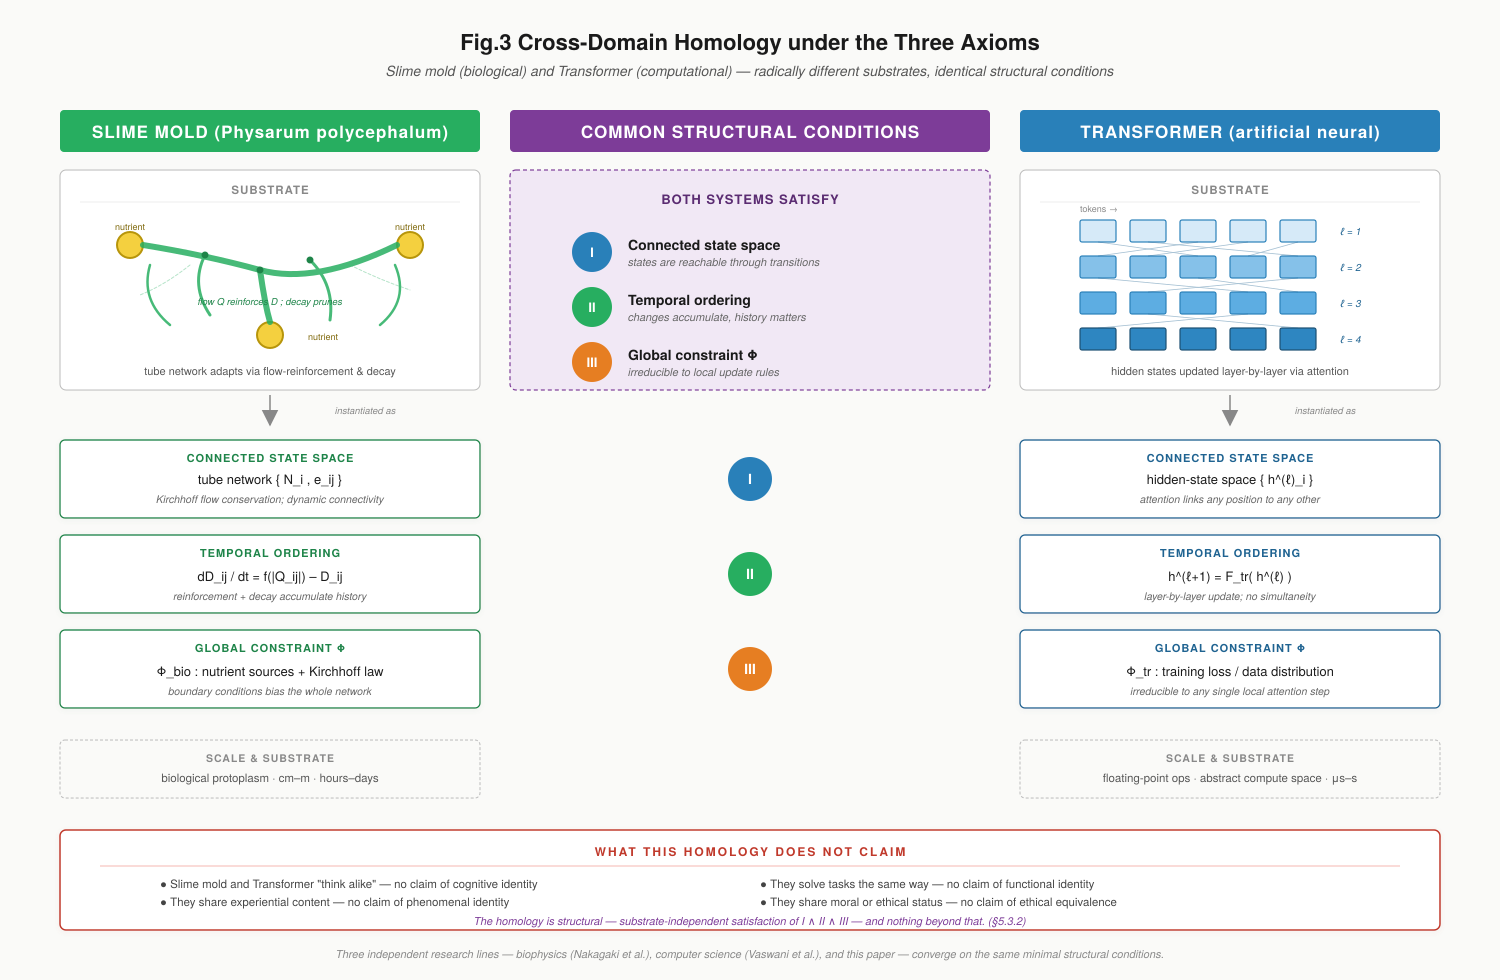
\includegraphics[width=\textwidth]{figures/fig3_cross_domain_homology.png}
\caption{Cross-domain homology under the three axioms. Slime mold and Transformer systems differ radically in substrate but satisfy the same minimal structural conditions.}
\label{fig:intelligence_part1_3}
\end{figure}
